%%%%%%%%%%%%%%%%%%%%%%%%%%%%%%%%%%%%%%%%%%%%%%%%%%%%%%%%%
% Niniejszy plik przedstawia przykładowy skład 
% pracy dyplomowej na Wydziale Matematyki PWr. 
% 
% Autorzy: 
% Damian Fafuła
% Michał Kijaczko
% Jakub Michalczak
% Maciej Miśta
% Dagmara Nowak
% Tomasz Skalski
% Wojciech Słomian
%
%% Data utworzenia: 8.05.2018
% Numer wersji: 1
%
% Poniższą formatkę można rozpowszechniać i edytować 
% pod warunkiem zachowania numeru wersji, 
% informacji o autorach i dodaniu informacji 
% o wprowadzonych zmianach.
%
%%%%%%%%%%%%%%%%%%%%%%%%%%%%%%%%%%%%%%%%%%%%%%%%%%%%%%%%%
% Domyślną opcją jest: praca magisterska, język polski.
% W przypadku pracy pisanej w języku angielskim dodajemy 
% opcję [english].
% Dla pracy licencjackiej dodajemy opcję [licencjacka].
% Dla pracy inżynierskiej dodajemy opcję [inzynierska].
% Dopuszczalne są podwójne opcje, np. [licencjacka, english].
% Opcje dodajemy w kwadratowym nawiasie przy \documentclass.
%
%
%%%%%%%%%%%%%%%%%%%%%%%%%%%%%%%%%%%%%%%%%%%%%%%%%%%%%%%%%
\documentclass[inzynierska]{pwr_wmat_praca_dyplomowa}
%%%%%%%%%%%%%%%%%%%%%%%%%%%%%%%%%%%%%%%%%%%%%%%%%%%%%%%%%
%              DANE DO PRACY
%
% W przypadku pracy dyplomowej w języku angielskim nie jest konieczne 
% wypełnianie pól: \tytul{}, \kierunek{}, \specjalnosc{}, 
%                  \streszczenie{}, \slowakluczowe{}.
%%%%%%%%%%%%%%%%%%%%%%%%%%%%%%%%%%%%%%%%%%%%%%%%%%%%%%%%%
%
% Imię i nazwisko autora
\autor{Aleksander Jakóbczyk}
%
% Tytuł pracy dyplomowej 
\tytul{Zastosowanie stochastycznej
	optymalizacji do gier
	częściowo obserwowalnych} 
\tytulang{Tytuł pracy dyplomowej w języku angielskim}
%
% Tytuł / stopień / imię i nazwisko opiekuna
\opiekun{dr inż. Andrzej Giniewicz}
%
% Kierunek studiów wybieramy spośród następujących:
% 1) Matematyka
% 2) Matematyka i Statystyka
% 3) Matematyka stosowana
\kierunekstudiow{Matematyka stosowana}
%
% Kierunek studiów po angielsku wybieramy spośród następujących:
% 1) Mathematics
% 2) Mathematics and Statistics
% 3) Applied Mathematics
\kierunekstudiowang{Mathematics}
%
% Specjalność wybieramy spośród następujących: 
% KIERUNEK: Matematyka
% 1) Matematyka teoretyczna,
% 2) Statystyka matematyczna,
% 3) Matematyka finansowa i ubezpieczeniowa,
%
% KIERUNEK: Matematyka i Statystyka
% 4) Matematyka,
% 5) Statystyka i analiza danych, 
%
% 6) -- (w przypadku braku specjalizacji).
\specjalnosc{--} 
%
% Specjalność w języku angielskim wybieramy spośród następujących:
% KIERUNEK: Matematyka
% 1) Theoretical Mathematics,
% 2) Mathematical Statistics,
% 3) Financial and Actuarial Mathematics,
%
% KIERUNEK: Matematyka i Statystyka
% 4) Mathematics,
% 5) Statistics and Data Analysis,
%
% KIERUNEK: Applied Mathematics
% 6) Financial and Actuarial Mathematics, 
% 7) Mathematics for Industry and Commerce,
% 8) Computational Mathematics,
% 9) Modelling, Simulation and Optimization.
%
% 10) -- (w przypadku braku specjalizacji).
\specjalnoscang{Theoretical Mathematics} 
%
% Krótkie streszczenia po polsku i angielsku
% - nie dłuższe niż 530 znaków.
\streszczenie{Celem rozprawy jest wyznaczenie nieoczekiwanych strategii w grach częściowo obserwowalnych za pomocą metod
	stochastycznej optymalizacji. Praca będzie opierać się na wynikach Cauwet i Teytauda z 2018 roku, w których
	przedstawili nieoczekiwane strategie dla kilku klasycznych gier oraz kilku metod optymalizacji. Podjęta zostanie
	próba odtworzenia oraz rozszerzenia wyników na kolejną grę. Przeprowadzona zostanie analiza porównawcza dla
	różnych metod optymalizacji.}
\streszczenieang{Tutaj piszemy krótkie streszczenie pracy w języku angielskim (nie powinno być dłuższe niż 530 znaków).}
%
% Podajemy najważniejsze słowa kluczowe po polsku i angielsku
% - w obu przypadkach, nie więcej niż 150 znaków.
\slowakluczowe{tutaj podajemy najważniejsze słowa kluczowe (łącznie nie powinny być dłuższe niż 150 znaków).}  
\slowakluczoweang{tutaj podajemy najważniejsze słowa kluczowe w języku angielskim (łącznie nie powinny być dłuższe niż 150 znaków)}
%
%
%%%%%%%%%%%%%%%%%%%%%%%%%%%%%%%%%%%%%%%%%%%%%%%%%%%%%%%%%
% Definicje, lematy, twierdzenia, przykłady i wnioski
% Komendy wywołujące twierdzenia, definicje, itd., 
% czyli 'theorem', 'definition', 'corollary', itd., 
% można zmienić wedle uznania.
\theoremstyle{plain}
\newtheorem{theorem}{Twierdzenie}
\numberwithin{theorem}{chapter}
\newtheorem{lemma}[theorem]{Lemat} 
\newtheorem{corollary}[theorem]{Wniosek}
\newtheorem{fact}[theorem]{Fakt}
\theoremstyle{definition}
\numberwithin{theorem}{chapter}
\newtheorem{definition}[theorem]{Definicja} 
\newtheorem{example}[theorem]{Przykład}
\newtheorem{note}[theorem]{Uwaga}
%%%%%%%%%%%%%%%%%%%%%%%%%%%%%%%%%%%%%%%%%%%%%%%%%%%%%%%%%

\usepackage{amsmath}
\usepackage{amsthm}
\usepackage{amsfonts}
\usepackage{amssymb}
\usepackage{graphicx}
\usepackage{caption}
\usepackage{xcolor}
\usepackage{algpseudocode,algorithm,algorithmicx}
\usepackage{enumitem}
\usepackage[plmath]{polski}
%icomma
\DeclareRobustCommand{\bbone}{\text{\usefont{U}{bbold}{m}{n}1}}
\DeclareMathOperator{\EX}{\mathbb{E}}% expected value
\DeclareCaptionLabelFormat{custom2}
{%
	#1 \thealgorithm:
}

%%%%%%%%%%%%%%%%%%%%%%%%%%%%%%%%%%%%%%%%%%%%%%%%%%%%%%%%%
%%%%%%%%%%%%%%%%%%%%%%%%%%%%%%%%%%%%%%%%%%%%%%%%%%%%%%%%%
\begin{document}
\frontmatter
\maketitle
\mainmatter
\tableofcontents
%\listoffigures
%\listoftables

{\backmatter \chapter{Wstęp}}
%We wstępie zapowiadamy, o czym będzie praca. Próbujemy zachęcić czytelnika do dalszej lektury, np. krótko informując, dlaczego wybraliśmy właśnie ten temat i co nas w nim zainteresowało.

%\chapter{Rozdział pierwszy}
%Tabela \ref{tab:przykladowa} przedstawia przykładową tabelę. Do tworzenia tabeli służą m.in. środowiska \texttt{tabular} oraz \texttt{table}. Istnieje możliwość numeracji dwustopniowej, gdzie pierwsza cyfra oznacza numer rozdziału, a druga – kolejny numer tabeli w tym rozdziale. Tytuł powinien znajdować się centralnie nad tabelą, $12$ pkt odstępu od tekstu zasadniczego nad i pod tabelą wraz z tytułem. Jeśli tabela jest cytowana – należy podać centralnie pod tabelą źródło jej pochodzenia, np. opracowanie własne, opracowano na podstawie danych z GUS.
%\begin{table}[ht]
%\caption{Podstawowa Tabela}
%\centering
%\begin{tabular}{ccc}
%\hline
%\hline                       
%Państwo & PKB (w milionach USD )& Stopa bezrobocia  \\  [0.5ex] 
%\hline 
%Stany Zjednoczone & 75 278 049 & 4,60\%  \\
%Chiny & 11 218 281 & 4,10\%   \\
%Japonia & 4 938 644 & 3,10\%  \\
%Niemcy & 3 466 639 & 6,00\%   \\
%Wielka Brytania & 2 629 188 & 4,60\%  \\ [1ex]  
%\hline 
%\end{tabular}
%\caption*{\textit{Źródło: opracowanie własne}}
%\label{tab:przykladowa} 
%\end{table}
%
%%Do cytowania używamy komendy \texttt{cite}. W nawiasie klamrowym podajemy klucz, którego użyliśmy w pliku \emph{bibliografia.bib}. Przykład: \cite{einstein} lub \cite[chap. 2]{latexcompanion}.
%
%\section{Podrozdział pierwszy}
%
%\begin{table}[H]
%\caption{Podstawowa Tabela}
%\centering
%\begin{tabular}{ccc}
%\hline
%\hline                       
%Państwo & PKB (w milionach USD )& Stopa bezrobocia  \\  [0.5ex] 
%\hline 
%Stany Zjednoczone & 75 278 049 & 4,60\%  \\
%Chiny & 11 218 281 & 4,10\%   \\
%Japonia & 4 938 644 & 3,10\%  \\
%Niemcy & 3 466 639 & 6,00\%   \\
%Wielka Brytania & 2 629 188 & 4,60\%  \\ [1ex]  
%\hline 
%\end{tabular}
%\caption*{\textit{Źródło: opracowanie własne}}
%\label{tab:przykladowa2} 
%\end{table}
%
%\section{Podrozdział drugi}
%
%Rysunki do pracy dyplomowej należy wstawiać w sposób podobny do wstawiania tabel, z~zasadniczą różnicą polegającą na tym, że podpis powinno umieszczać się centralnie pod rysunkiem, a nie powyżej niego. Numeracja i sposób cytowania pozostają bez zmian, przy czym tabele i rysunki nie mają numeracji wspólnej, np. po Tabeli \ref{tab:przykladowa2} występuje Rysunek \ref{rys1} (o ile jest to pierwszy rysunek rozdziału pierwszego), a nie Rysunek $1.3$.
%
%\begin{figure}[ht]
%
%\centering
%                     
%
\includegraphics[scale=0.27]{logo_w13.jpg}
%\caption{Podstawowy Rysunek}\label{rys1}
%\end{figure}
%\label{rys:przykladowy} 


\chapter{Definicje, lematy, twierdzenia, przykłady i wnioski}
Celem algorytmów, których będziemy wykorzystywać, jest znalezienie optymalnej strategi w dwuosobowych grach częściowo obserwowalnych. Zdefiniujmy zatem podstawowe pojęcia potrzebne nam do tego, aby matematycznie opisać czym jest gra i czym jest strategia optymalna.
W tym celu wprowadzimy kilka podstawowych definicji.
Definicje dotyczące podstawy teorii gier  pochodzą z \cite{platkowski2012wstkep},\cite{prisner2014game}.

\section{Typy gier }
Podstawową kategorią, na jaką możemy podzielić gry, jest podział ze względu na czas, w którym gracze podejmują decyzje:
%\begin{definition}[Gra]
%Gra w matematycznym sensie jest sytuacja, w której gracze podejmują  decyzje zgodnie z określonymi zasadami w celu uzyskania jakiejś wypłaty.
%\end{definition}
\begin{definition}[Gra w postaci strategicznej]
Jest to typ gry, w której gracze podejmują decyzje w tym samym
momencie.
\end{definition}
\begin{definition}[Gra w postaci ekstensywnej]
	Jest to typ gry, w której gracze podejmują decyzje we wcześniej
	ustalonej kolejności.
\end{definition}
Przykładami gier w postaci strategicznej są gry kamień papier nożyce, oszust czy też mora. Natomiast przykładami gier w postaci ekstensywnej są szachy, warcaby oraz go.

Gry możemy również dzielić ze względu na posiadaną wiedzę.
\begin{definition}[Gra z kompletną informacją]
	Jest to typ gry, w której gracze mają informacje o możliwych
	przyszłych wynikach gry i o zbiorach możliwych strategii.
\end{definition}
\begin{definition}[Gra częściowo obserwowalna]
	Jest to przeciwnie gier z kompletną informacją.
\end{definition}
Przykładami gier z kompletną informacją są szachy, warcaby oraz go.
Natomiast przykładami gier częściowo obserwowanymi są wszelkie gry posiadające w rozgrywce pewien elementy losowe takie jak rzut kostką czy też dobieranie kart. 

Istnieje jeszcze wiele innych podziałów gier ze wglądu na kategorie takie jak liczba graczy,zbiory dostępnych akcji, możliwość tworzenia koalicji i wiele innych.

\section{Definicje i Oznaczenia}
\subsection{Strategie proste}
Wprowadźmy podstawowe oznaczenia potrzebne nam do tego, aby móc zdefiniować czym jest strategia optymalna.
\begin{itemize}
	\item $ N = \{1,2,\dots, n\} $ -- zbiór graczy,
	\item $A_i,\; i \in N $ -- niepusty zbiór strategii  czystych gracza $i$,
	\item $m_i = |A_i|$ -- liczba strategi gracza $i$,
	\item $A = \displaystyle\prod_{i \in N} A_i$ -- zbiór wszystkich strategii gry, 
	\item $u_i : A \rightarrow \mathbb{R} $ -- funkcja wypłaty gracza $i$,
	\item $a=(a_1,a_2,\dots,a_n)=(a_i)_{i \in N},\; a_i \in A_i$ -- profil gry w strategiach czystych,
	\item $u_i(a) = u_i(a,a_{-i})$ -- wypłata gracza $i$ z profilu $a$,
	\item $a_{-i} = (a_i)_{i\in N \setminus \{i\}}$, -- profil wszystkich strategii poza strategią graca $i$.
\end{itemize}
	\begin{definition}[Gra strategiczna]
		Grą strategiczną nazywamy trójkę $GS = \langle N, (A_i)_{i \in N},(u_i)_{i \in N} \rangle $.
	\end{definition}
	
	\begin{definition}[Równowaga Nasha w strategiach czystych gry strategicznej]
		Równowaga Nasha w strategiach czystych gry strategicznej jest to profil gry $a^*= (a_1^*,a_2^*,\dots,a_N^*)\in A$, takim, że:
		\begin{align*}
			\mathop{\forall}{i \in N}\;
			\mathop{\forall}{a_i \in A_i} \quad
			u_i(a_i^*,a_{-i}^*) \ge u_i(a_i, a_{-i}^*)
		\end{align*}
	\end{definition}
	Zatem jest to profil gry, w którym istnieje strategia czysta dająca nie gorsze wyniki od dowolnej innej strategii czystej.
	Okazuje się jednak, że taki stan nie zawsze istnieje w strategiach czystych, np. w grze kamień papier nożyce strategia grania tylko kamienia daje gorsze rezultat przeciwko graniu tylko papieru. Podobnie ze strategią grania tylko nożyc i grania tylko papieru.
	\subsection{Strategie mieszane}
	\begin{definition}[Strategia mieszana]
		Strategia mieszana $\sigma_i$ graca $i$ w grze strategicznej $GS = \langle N, (A_i)_{i \in N},(u_i)_{i \in N} \rangle $. Nazywamy rozkład prawdopodobieństwa na zbiorze strategi czystych $A_i$:
		\begin{align*}
			\sigma_i = (\sigma_{i1}, \sigma_{i2},\dots,\sigma_{im_i})
		\end{align*}
	gdzie $\sigma_{ik}$ oznacza prawdopodobieństwo, że gracz $i$ zagra strategie czysta $k\in A_i$.  
	\end{definition}

	\begin{fact}
		Strategia czysta jest szczególnym przypadkiem strategij mieszanej, w którym prawdopodobieństwo zagrania jednej z dostępnych strategii wynosi 1.
	\end{fact}
	Wprowadźmy dodatkowe oznaczenia:
 	\begin{itemize}
 		\item $\Sigma_i  = \left\{ \sigma_i: A_i \rightarrow [0,1],\displaystyle\sum_{k=1}^{n} \sigma_{ik} = 1, \sigma_{ki}\ge 0 \right\}$ -- zbiór strategii mieszanych gracza $i$,
 		\item  $\sigma = (\sigma_1, \sigma_2,\dots,\sigma_n)$ -- profil gry,
 		\item $u_i(\sigma) = u_i(\sigma_i,\sigma_{-i})$ -- wypłata gracza $i$ z profilu $\sigma$,
 		\item $\sigma_{-i} = (\sigma_i)_{i\in N \setminus \{i\}}$, -- profil wszystkich strategii poza strategią graca $i$. 
 	\end{itemize}
	\begin{definition}[Równowaga Nasha w strategiach mieszanej gry strategicznej]
		Profil gry strategicznej $\sigma_i^*$ jest Równowagą Nasha gdy:
		\begin{equation*}
			\mathop{\forall}{i \in N}\;
			\mathop{\forall}{\sigma_i \in \Sigma_i} \quad
			u_i(\sigma_i^*,\sigma_{-i}^*) \ge u_i(\sigma_i, \sigma_{-i}^*)
		\end{equation*}
	Równowaga Nasha interpretujemy jako taki profil gry, w którym żaden z graczy nie opłaca się zmieniać swojej strategi, ponieważ nie skutkuje to zwiększeniem swoich zysków.
	\end{definition}

	\section{Twierdzenia}
	Algorytmy \ref{alg:LEBR}, \ref{alg:LEBR 1}, \ref{alg:LEBR 2}, \ref{alg:IEBLR* 1}, \ref{alg:IEBLR* 2} wykorzystywane w poniższej pracy oparte są o dwa twierdzenia a dokładniej o szczególne przypadki wynikające z nierówności \ref{Hoffding ineq} i \ref{Bernsteina emp ineq}:
	\begin{theorem}[Nierówność Hoffdinga]
		\label{Hoffding ineq}
		Niech $X_1,X_2,\dots,X_t$ będzie ciągiem niezależnych zmiennych losowych (i.i.d.) takim, że $a_i \le X_i \le b_i$, wtedy:
		\begin{gather*}
			S_t = \sum_{i=1}^{t} X_i,\quad c_i = b_i - a_i, \\
			P(|S_t - \EX(S_t)| \ge \epsilon ) \le 2\exp\left( -\frac{2\epsilon^2}{\sum_{i=1}^{n} c_i^2} \right)
		\end{gather*}
	\end{theorem}
	\begin{lemma}
		\label{Hoffding ineq lemma}
		Niech $X_1,X_2,\dots,X_t$ będzie ciągiem niezależnych zmiennych losowych (i.i.d.) takim, że $0 \le X_i \le 1$, wtedy:
		\begin{gather*}
			\overline{X}_t = \frac{S_t}{t},\quad 
			\mu = \EX(X_i),\quad  	
			P(|\overline{X}_t - \mu | \le \epsilon ) = 1 - \delta, \\
			\epsilon \le  \sqrt{\frac{\ln(2/\delta)}{2t}}   
		\end{gather*}
	\end{lemma}

		\begin{theorem}[Empiryczna nierówność Bernsteina]
		\label{Bernsteina emp ineq}
		Niech $X_1,X_2,\dots,X_t$ będzie ciągiem niezależnych zmiennych losowych (i.i.d.) takim, że $a \le X_i \le b$, wtedy:
		\begin{gather*}
			P(|\overline{X}_t - \mu| \ge \epsilon ) \le  \delta, \quad \overline \sigma_t^2 = \frac{1}{t}\sum_{i=i}^{t}(X_i - \overline{X}_t)^2, \\
			|\overline{X}_t - \mu | \le \overline{\sigma}_t \sqrt{\frac{2\ln(3/\delta)}{t}} + \frac{3 R \ln{(3 / \delta)}}{t}
		\end{gather*}
	\end{theorem}
	\begin{lemma}\label{Bernsteina emp ineq lemma}
		Niech $X_1,X_2,\dots,X_t$ będzie ciągiem niezależnych zmiennych losowych (i.i.d.) takim, że $0 \le X_i \le 1$, wtedy:
		\begin{gather*}
			P(|\overline{X}_t - \mu | \le \epsilon ) = 1 - \delta,\\
			\epsilon \le \overline{\sigma}_t \sqrt{\frac{2\ln(3/\delta)}{t}} + \frac{3  \ln{(3 / \delta)}}{t}
		\end{gather*}
	\end{lemma}

	\section{Problem porównań wielokrotnych}
	Załóżmy, że z prawdopodobieństwem $1-\delta$ chcemy wiedzieć który z dwóch graczy, $p_1$ i $p_2$ jest lepszy. W tym
	celu będziemy przeprowadzać testy statystyczne, dla których
	prawdopodobieństwo pomyłki k-tego testu wynosi $\delta_k$, aż do momentu, gdy jeden z graczy wygra przeważającą ilość razy. Wtedy po przeprowadzeniu $n$ takich testów
	\begin{gather*}
		P(\text{Chociaż jeden z $n$ testów się pomylił}) \overset{(*)}{\le} \sum_{k=1}^n \delta_k \implies  \\
	P(\text{Żaden test się nie pomylił}) \le 1 - \sum_{k=1}^n \delta_k,
	\end{gather*} 
	gdzie nierówność oznaczona $(*)$ wynika z faktu, że $P(X+Y) \le P(X) + P(Y)$.
	
	Oznacza to, że musimy wprowadzić pewną korektę, aby
	ostateczne prawdopodobieństwo popełnienia błędu było
	mniejsze niż $\delta$.
	Możemy zastosować jedna z dwóch poprawek:

	\begin{enumerate}[label=\thesection.\arabic*]
		\item \label{korekta 1} Niech $n$ będzie maksymalną liczbą testów jaką pozwalamy wykonać, aby wyznaczyć lepszego
		gracza. Wtedy $\delta_k=\frac{\delta}{n}$.
		\item \label{korekta 2} Niech $\delta_k$ spełnia nierówność $ \delta \ge \sum_{k = 1}^{\infty}\delta_k$. Wtedy niezależnie od
		ilości przeprowadzonych testów, ostateczne
		prawdopodobieństwo pomyłki będzie nie większe niż~$\delta$.
	\end{enumerate}

	\section{Algorytmy wyścigowe}
	Jednymi z algorytmów stosującymi dane korekty są algorytmy wyścigowe
	(\selectlanguage{english}{Racing Algorytms}). Dwoma najpopularniejszymi typami algorytmów racingowych są ,,Hoffding race'' oraz ,,Bernstein race''.
	Oparte są one odpowiednio o Twierdzenie \ref{Hoffding ineq} i Twierdzenie \ref{Bernsteina emp ineq lemma} oraz korektę \ref{korekta 2} . Mają one jednak pewną wadę, mogą trwać one dużą ilość czasu, a w momencie, gdy poziom umiejętności porównywanych graczy jest sobie równy (prawdopodobieństwo wygranej wynosi 50\%), wtedy z prawdopodobieństwem równym $1-\delta$ algorytm się nigdy nie zatrzyma.
	
	W celu poradzenia sobie z problemami, jakie wiążą się z klasycznymi algorytmami wyścigowymi, wprowadzimy  tzw. Limited Racing algorytm. Załóżmy zatem dodatkowy warunek, który mówi, że przerywamy działanie algorytmu w momencie, gdy empiryczna wartość oczekiwana z prawdopodobieństwem większym bądź równym $1-\delta$ jest znana z dokładnością co do zadanego $\epsilon$. W poniższej pracy będziemy przyjmować $\epsilon=0.01$ oraz $\delta = 0.05$.
	\subsection{Algorytm Limited Empirical Bernstein Race (LEBR)}
	Klasyczny algorytm racingowy opiera się na szeregu $\epsilon_t$ który posiada właściwość że zdarzenie $\mathcal{E}= \{|\overline{X}_t - \mu | \le \epsilon_t,\; t\in \mathbb{N}^+\}$ występuje z prawdopodobieństwem nie mniejszym 
	\\niż $1-\delta$. Niech $\delta_k$ będzie dodatnim szeregiem spełniającym $ \delta \ge \sum_{k = 1}^{\infty}\delta_k$ wtedy korzystając z Lematu \ref{Bernsteina emp ineq lemma}
	\begin{gather*}
		\label{eq:LEBR epsilon}
		\epsilon_t =  \overline{\sigma}_t \sqrt{\frac{2\ln(3/\delta_t)}{t}} + \frac{3  \ln{(3 / \delta_t)}}{t}
	\end{gather*}
	Ponieważ $\delta_k$ sumuje się co najmniej do $\delta$ oraz $(\overline{X}_t - \epsilon_t, \overline{X}_t + \epsilon_t)$ jest przedziałem ufności dla $\mu$ o współczynniku ufności $1-\delta_t$ 
	otrzymanym z Lematu \ref{Bernsteina emp ineq lemma}, uzyskujemy że zdarzenie $\mathcal{E}$ występuję z prawdopodobieństw nie mniejszym niż $1-\delta$. Identyczny rezultat otrzymujemy stosując $\epsilon_t$ oparte o Lemat \ref{Hoffding ineq lemma} jednak zmienia się wtedy postać $\epsilon_t$. W pracy \cite{cauwet2018surprising} algorytm opierał się o szereg $\delta_t=\frac{c\delta_t}{t^2},\; c=\frac{6}{\pi^2}$.
	Pseudo kod jest pokazany jako Algorytm \ref{alg:LEBR} omówmy zarys metody. Rozgrywamy $t$ gier, i wyznaczamy granice górna $\text{UB} = \displaystyle\min_{1\le k\le t}( \overline{X}_k+c_k)$  oraz granice dolną $\text{LB} = \max(0,\displaystyle\max_{1\le k\le t}(\overline{X}_k-c_k))$. Algorytm kończy się w momencie gdy $\text{UB}-\text{LB}< 2\epsilon$. Otrzymane w ten sposób $\overline{X}$ z prawdopodobieństwem nie mniejszym niż $1 - \delta$ wynosi $\mu$ z dokładnością co zadanego $\epsilon$. 
	\begin{algorithm}[H]
		\caption{LEBR}\label{alg:LEBR}
		\begin{algorithmic}
			\Ensure precision $\epsilon$, probabilitys $\delta_k$
			\State $LB \gets 0, \quad UB \gets \infty, \quad t \gets 0,\quad n \gets 1$ 
			\While{$ UB - LB > 2\epsilon $} 
			\State $t \gets t + 1$
			\State Obtain $X_t$				
			\State $\epsilon_n \gets \overline{\sigma}_n \sqrt{\frac{2\ln(3/\delta_n)}{n}} + \frac{3  \ln{(3 / \delta_n)}}{n}$ 
			\State $LB \gets \max(LB,  \overline{X_n} - \epsilon_n)$
			\State $UB \gets \min(BU,  \overline{X_n} + \epsilon_n)$
			\State $n \gets n + 1$
			\EndWhile
			\State \Return $ \overline{X_t}$		
		\end{algorithmic}
	\end{algorithm}

	\subsection{Improved LEBR (ILEBR)}
	Algorytm \ref{alg:LEBR} opiera się na korekcie \ref{korekta 2} która zakłada możliwie nieskończoną ilość testów. Jednak dołożenie ograniczenia na temat żądanej dokładności rzędu $\epsilon$ pozwala nam znaleźć maksymalną ilość testów jaką należy wykonać aby z prawdopodobieństwem nie mniejszym niż $1-\delta$ empiryczna wartość oczekiwana była równa teoretycznej wartości oczekiwanej z dokładnością co do $\epsilon$. Niech $\delta_k = \frac{\delta}{n_{max}}$ gdzie $n_{max}$ oznacza maksymalną potrzebną ilość testów. Z Lematu \ref{Hoffding ineq lemma} niezależnie od odchylenia standardowego zmiennej losowej $X_i$ jesteśmy w stanie oszacować $n_{max}$ rozwiązując analitycznie poniższe równie \ref{eq:ILEBR Hoffdin}
	\begin{gather}
		\label{eq:ILEBR Hoffdin}
		\epsilon =  \sqrt{\frac{\ln(2n_{max}/\delta)}{2n_{max}}} 
	\end{gather}

	Dla $\epsilon=0.01$ i $\delta=0.05$ rozwiązaniem numerycznym równania \ref{eq:ILEBR Hoffdin} jest $n_{max}=74539.85$.
	Oznacza to że maksymalna ilość gier jaką  należy rozegrać między dwoma graczami aby z prawdopodobieństwem nie mniejszym niż $1-0.05$ oszacować prawdopodobieństwo wygrania gry przez pierwszego gracza z dokładniejsi co do $0.01$ wynosi $\lceil n_{max} \rceil = 74540$. 
	   
	Podobnie możemy postąpić w przypadku nierówności Bernsteina.
	Na początku jednak musimy oszacować z góry $\overline{\sigma}_t$.
	Przyjmijmy, że $X_i$ jest zmienną z rozkładu zero-jedynkowego.
	Wtedy maksymalna możliwa wariancja dla takiej zmiennej losowej wynosi $\sigma^2 = 0.5$. Jest to również maksymalna możliwa wartość dla naszej empirycznej wariancji. Podstawiając wtedy $\delta_n = \frac{0.05}{n}, \epsilon = 0.01$ do Lematu \ref{Bernsteina emp ineq lemma} otrzymujemy:
	\begin{gather}
		\label{eq:ILEBR Bernstein}
		0.01 \le \sqrt{\frac{\ln(\frac{3n_{max}}{0.05})}{n_{max}}} + \frac{3  \ln(\frac{3n_{max}}{0.05})}{n_{max}} 
	\end{gather}
	Rozwiązaniem numerycznym równania \ref{eq:ILEBR Bernstein} jest $n_{max}=170986$. Jednak granice oparte o nierówność Bernsteina zalezą od wariancji. Sprawdźmy zatem jak wygląda $n_{max}$ w zalotności od $\sigma^2$.
	\begin{figure}
		\centering
		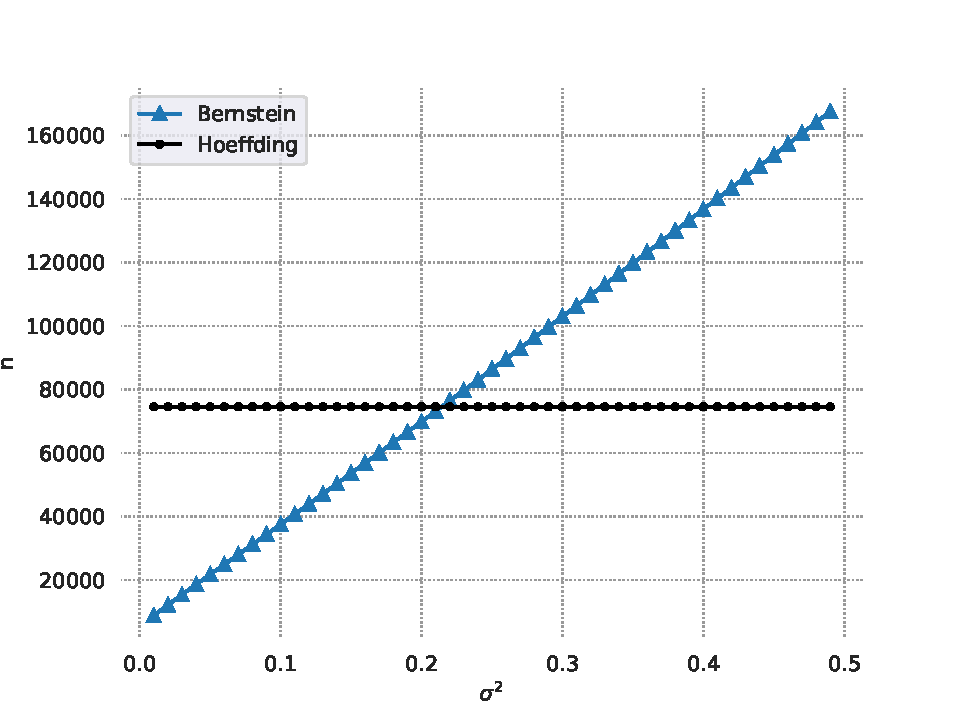
\includegraphics[width=0.75\textwidth]{imagens/t_eq_n.pdf}
		%latinmodern w pythonie
		\caption{Wykres maksymalnej potrzebnej ilości testów w zależności od wariancji zmiennych losowych  $X_i$ w przypadku gdy liczba testów jest równa liczbie gier ($t = n$) dla $\epsilon=0.01$ i $\delta = 0.05$.}
		\label{fig:t_eq_n}
	\end{figure}
	Z Rysunku \ref{fig:t_eq_n} widzimy zatem, że algorytm oparty o nierówność Bernsteina radzi sobie lepiej w przypadku gdy niskiej wariancji. Co więcej niezależnie od ilości wykonywanych testów, dla $\delta_n = \frac{0.05}{74540}$ maksymalna ilość gier po której z prawdopodobieństwem $1-0.05$ wiemy że $|\overline{X_i} - \mu| \le 0.01$ wynosi $74540$. Oznacza to że do Algorytmu \ref{alg:LEBR} możemy zastosować funkcje $\epsilon_k$ opartą o $\delta_k = \frac{\delta}{n_{max}}$ oraz dołożyć nowy warunek zatrzymania algorytmu gdy liczba wykonanych testów przekroczy $n_{max}$. Dotychczas uwzględnione poprawki przedstawione sa przy Algorytmu \ref{alg:LEBR 1}.
	\begin{algorithm}[H]
		\caption{ILEBR 1}\label{alg:LEBR 1}
		\begin{algorithmic}
			\Ensure precision $\epsilon$, probability $\delta$
			\State $LB \gets 0, \quad UB \gets \infty, \quad t \gets 0,\quad n \gets 1$
			\State Find $n_{max}$ such as $		\epsilon =  \sqrt{\frac{\ln(2n_{max}/\delta)}{2n_{max}}} $
			\Statex $\delta_n = \delta/n_{max}$
			\While{$ UB - LB > 2\epsilon $ or $n<n_{max}+1$}  
			\State $t \gets t + 1$
			\State Obtain $X_t$
			\State $\epsilon_n \gets \overline{\sigma}_n \sqrt{\frac{2\ln(3/\delta_n)}{n}} + \frac{3  \ln{(3 / \delta_n)}}{n}$ 
			\State $LB \gets \max(LB,  \overline{X_n} - \epsilon_n)$
			\State $UB \gets \min(BU,  \overline{X_n} + \epsilon_n)$
			\State $n \gets n + 1$
			\EndWhile
			\State \Return $ \overline{X_t}$		
		\end{algorithmic}
	\end{algorithm}
	Algorytmy \ref{alg:LEBR} i \ref{alg:LEBR 1} przeprowadzały testy po każdej rozegranej grzęz, skutkuje to wytopieniem bardzkiej ilości testów. Zamiast przeprowadzać test po każdej rozegranej grze, niech test odbywa się w momencie gdy liczba rozegranych gier będzie równa pewnej funkcji zależnej od ilości przeprowadzonych testów. Na podstawie artykuł \cite{heidrich2011non} wiemy że funkcja która pozwoli nam na polepszenie wyników jest $t = n^2$. Przeprowadźmy identyczną procedure jak w przypadku równań \ref{eq:ILEBR Hoffdin} i \ref{eq:ILEBR Bernstein}. Tym razem jednak zamiast stosować $t = n$ do Lematów \ref{Hoffding ineq lemma} i \ref{Bernsteina emp ineq lemma}  zastosujmy $t = n^2$.
	
	W przypadku granicy opartej o nierówność Hoffdina otrzymujemy
	\begin{gather}
		\label{eq:ILEBR Hoffdin t=n^2}
		\epsilon =  \sqrt{\frac{\ln(2n_{max}/\delta)}{2n_{max}^2}} \implies t_{max} = \lceil n_{max} \rceil^2 = \lceil213\rceil^2= 45369.
	\end{gather}
	W przypadku granicy opartej o nierówność Bernsteina otrzymujemy
	\begin{gather}
		\label{eq:ILEBR Bernstein t=n^2}
		0.01 \le \sqrt{\frac{\ln(\frac{3n_{max}}{0.05})}{n_{max}^2}} + \frac{3  \ln(\frac{3n_{max}}{0.05})}{n_{max}}^2\implies t_{max} = \lceil n_{max} \rceil^2 = \lceil324^2\rceil= 104976. 
	\end{gather}
	\begin{figure}
		\centering
		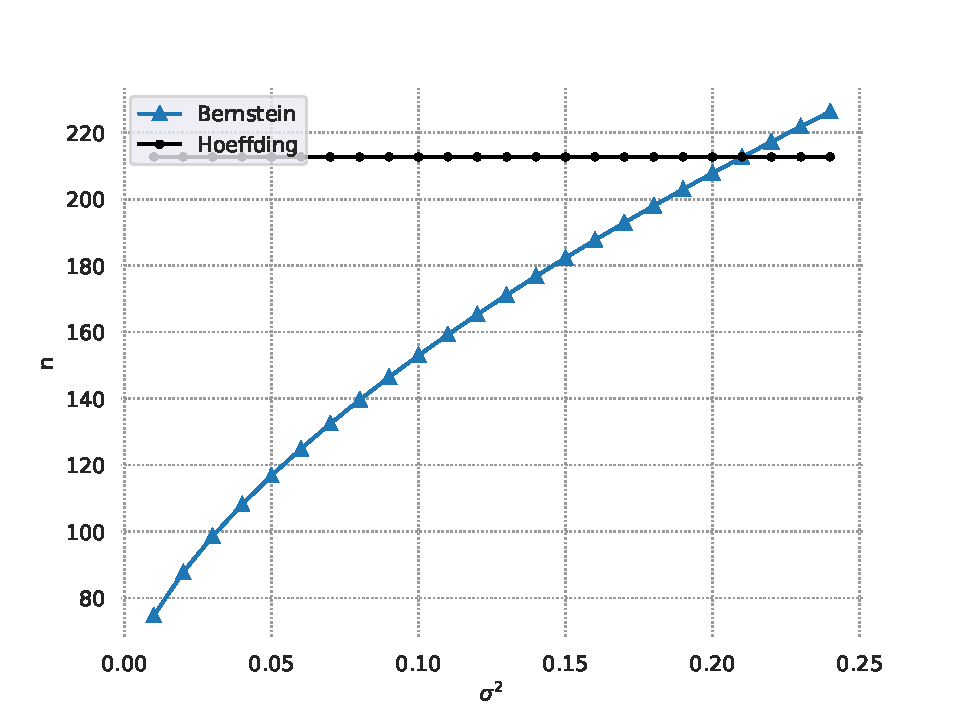
\includegraphics[width=0.8\textwidth]{imagens/t_eq_n_q.pdf}
%		\captionsetup{justification=centering}
		\caption{Wykres maksymalnej potrzebnej ilości testów w zależności od wariancji zmiennych losowych  $X_i$ w przypadku gdy liczba rozegranych gier jest równa liczbie przeprowadzonych testów do kwadratu ($t = n^2$) dla $\epsilon=0.01$ i $\delta = 0.05$.}
		\label{fig:t_eq_n_q}
	\end{figure}
	Porównując ze sobą uzyskane wartość z wzoru \ref{eq:ILEBR Hoffdin} oraz \ref{eq:ILEBR Hoffdin t=n^2} widzimy że udało się zmniejszyć maksymalną ilość gier jakie należny wykonać z 74540 do 45369.
	Wprowadźmy zatem nowo uzyskane poprawki trwożąc Algorytm \ref{alg:LEBR 2}.
	\begin{algorithm}[H]
		\caption{ILEBR 2}\label{alg:LEBR 2}
		\begin{algorithmic}
			\Ensure precision $\epsilon$, probability $\delta$
			\State $LB \gets 0, \quad UB \gets \infty, \quad t \gets 0,\quad n \gets 1$
			\State Find $n_{max}$ such as $		\epsilon =  \sqrt{\frac{\ln(2n_{max}/\delta)}{2n_{max}^2}} $
			\Statex $\delta_n = \delta/n_{max}$
			\While{$ UB - LB > 2\epsilon $ or $n<n_{max}+1$}  
			\Repeat 
			\State $t \gets t + 1$
			\State Obtain $X_t$
			\Until $t=n^2$
			\State $\epsilon_n \gets \overline{\sigma}_n \sqrt{\frac{2\ln(3/\delta_n)}{n^2}} + \frac{3  \ln{(3 / \delta_n)}}{n^2}$ 
			\State $LB \gets \max(LB,  \overline{X_n} - \epsilon_n)$
			\State $UB \gets \min(BU,  \overline{X_n} + \epsilon_n)$
			\State $n \gets n + 1$
			\EndWhile
			\State \Return $ \overline{X_t}$		
		\end{algorithmic}
	\end{algorithm}
	Do tej pory Wszystkie stosowane algorytmy wyznaczały nam prawdopodobieństwo wygranej pierwszego gracza. Jednak nam nie zależny na tym dokładnie znać prawdopodobieństwo wygranej graczy. Głównym celem algorytmów jest odnalezienie lepszego gracza. Pozwala nam to modyfikacje Algorytmu \ref{alg:LEBR 2} o nowe warunki zatrzymania.
	\begin{algorithm}[H]\captionsetup{labelformat=custom2}
		\caption{ILEBR* 1}\label{alg:IEBLR* 1}
		\begin{algorithmic}
			\Ensure precision $\epsilon$, probability $\delta$ 
			\State  $ LB \gets 0,\quad UB \gets \infty,\quad t \gets 1,\quad n \gets 0 $
			\State Find $n_{max}$ such as $		\epsilon =  \sqrt{\frac{\ln(2n_{max}/\delta)}{2n_{max}^2}} $
			\Statex $\delta_n = \delta/n_{max}$
			\While{$( UB - LB > 2\epsilon $ or $n < n_{max}+1)$ and $ (BU > 0.5 \text{ or } LB < 0.5)$}
			\Repeat 
			\State $t \gets t + 1$
			\State Obtain $X_t$
			\Until $t=n^2$
			\State $\epsilon_n \gets \overline{\sigma}_n \sqrt{\frac{2\ln(3/\delta_n)}{n^2}} + \frac{3  \ln{(3 / \delta_n)}}{n^2}$ 
			\State $LB \gets \max(LB,  \overline{X_n} - \epsilon_n)$
			\State $UB \gets \min(BU,  \overline{X_n} + \epsilon_n)$
			\State $n \gets n + 1$
			\EndWhile
			\If{$LB > 0.5$}
			\State \Return $p_1$ win
			\ElsIf{$UB < 0.5$}
			\State \Return $p_2$ win
			\ElsIf{$\overline{X_n} > 0.5$}
			\State \Return $p_1$ win
			\Else
			\State \Return $p_2$ win
			\EndIf
		\end{algorithmic}
	\end{algorithm}
	Do tej pory staraliśmy się ograniczyć z góry maksymalną ilość rozgrywanych gier. Jednak oczywistym faktem jest że nie ma sensu testowania który z graczy jest lepszy w monecie gdy ilość rozegranych gier jest niewystarczająco mały. Jadnak jak wyznaczyć nasze minimalne $t$ po którym zaczniemy testować? Algorytm oparte o nierówność Bernsteina najszybciej wyznaczają wynik w przypadku gdy wariancja naszej zmiennej losowej wynosi 0 (jeden z graczy zawsze wygrywa). Dla Algorytmu \ref{alg:IEBLR*} interesuje nas monet od którego będziemy w stanie rozróżnić kiedy dolna bać górna granica przekroczy $\frac{1}{2}$. Zatem oszacujmy $n_{min}$ korzystać z Lematu \ref{Bernsteina emp ineq lemma} dla $\overline{\sigma}_t=0$ i $t = n^2$.  
	
	
	
	\begin{gather*}
		\label{eq:ILEBR Bernstein t=n^2}
		0.5 \le \frac{3  \ln(\frac{3n_{min}}{0.05})}{n_{min}}\implies^2 t_{min} = \lceil n_{min} \rceil^2 = \lceil5.93749\rceil^2= 36. 
	\end{gather*}
	Oznacza to, że przy $\epsilon=0.01$ i $\delta= 0.05$ w przypadku gdy jeden graczy wygrywa zawsze, będziemy w stanie to stwierdzić nie prędzej niż po 36 grach.
	Na tej podstawie wyznaczy nowe $n_{max}$ uwzględniając pomijanie pierwsze niepotrzebne testy.
	\begin{gather}
		\label{eq:ILEBR Hoffdin t=n^2 and t_min}
		0.01 =  \sqrt{\frac{\ln(2n_{max}/0.05)}{2(n+6)_{max}^2}} \implies t_{max} = \lceil n_{max}+6\rceil^2 = \left\lceil 207+6\right\rceil^2= 45369.
	\end{gather}
	Chociaż równanie \ref{eq:ILEBR Hoffdin t=n^2 and t_min} nie zmniejszyło nam maksymalnej liczby testów jakie należy wykonać to pozwoliło nam ono na zmniejszenie $\epsilon_n$. Oznacza to że stosują odroczenie pierwszych testów, pozwala nam na dokładniejsze oszacowanie naszej górnej i dolnej granicy w stosowanych algorytmach.
	\begin{algorithm}[H]\captionsetup{labelformat=custom2}
		\caption{ILEBR* 2}\label{alg:IEBLR* 2}
		\begin{algorithmic}
			\Ensure precision $\epsilon$, probability $\delta$ 
			\State  $ LB \gets 0,\quad UB \gets \infty,\quad t \gets 1,\quad n \gets 0 $
			\State Find $n_{max}$ such as $		\epsilon =  \sqrt{\frac{\ln(2n_{max}/\delta)}{2(n+6)_{max}^2}} $
			\Statex $\delta_n = \delta/n_{max}$
			\While{$( UB - LB > 2\epsilon $ or $n < n_{max}+1)$ and $ (BU > 0.5 \text{ or } LB < 0.5)$}
			\Repeat 
			\State $t \gets t + 1$
			\State Obtain $X_t$
			\Until $t=n^2$
			\State $\epsilon_n \gets \overline{\sigma}_n \sqrt{\frac{2\ln(3/\delta_n)}{(n+6)^2}} + \frac{3  \ln{(3 / \delta_n)}}{(n+6)^2}$ 
			\State $LB \gets \max(LB,  \overline{X_n} - \epsilon_n)$
			\State $UB \gets \min(BU,  \overline{X_n} + \epsilon_n)$
			\State $n \gets n + 1$
			\EndWhile
			\If{$LB > 0.5$}
			\State \Return $p_1$ win
			\ElsIf{$UB < 0.5$}
			\State \Return $p_2$ win
			\ElsIf{$\overline{X_n} > 0.5$}
			\State \Return $p_1$ win
			\Else
			\State \Return $p_2$ win
			\EndIf
		\end{algorithmic}
	\end{algorithm}
	\newpage
	\subsection{Bernstein race without maximum race length}
	Wykorzystując Lemat~\ref{Bernsteina emp ineq lemma} oraz korektę \ref{korekta 2} z $\delta_k=\frac{c\delta}{k^2}, c=\frac{6}{\pi^2}$ otrzymujemy, że dla ciągu $X_1,X_2,\dots,X_t$ i.i.d. zmiennych losowych takim, że  $0 \le X_i \le 1$ 
	\begin{align*}
		\label{Bernstein race without maximum race length}
		\epsilon_{t,k} \le \overline{\sigma}_t \sqrt{\frac{2\ln(3/\delta_k)}{t}} + \frac{3  \ln{(3 / \delta_k)}}{t} =
		\overline{\sigma}_t\sqrt{\frac{2\ln(\frac{k^2\pi^2}{2\delta})}{t}} + \frac{3  \ln{(\frac{k^2\pi^2}{2\delta})}}{t}
	\end{align*}
	Wtedy $e_{t,k}$ interpretujemy jako maksymalną różnicę między empiryczną a teoretyczną wartością oczekiwaną po przeprowadzeniu $k$ testów i rozegraniu $t$ gier, z prawdopodobieństwem pomyłki równym 
	\begin{lemma}
		\label{lemma Bernstein race without maximum race length}
		Niech liczba rozegranych gier będzie funkcja zależną od k ($f(k) = t$) oraz niech $\delta_k = \frac{\delta}{g(k)}$
		gdzie $\delta \ge \sum_{k=1}^{\infty} \frac{\delta}{g(k)}$ i $\ln(g(k)) \in o(f(k))$. Wtedy
		$\lim\limits_{k\to\infty} e_{f(k),k} = 0$ 
	\end{lemma}
	\begin{proof}[Dowód Faktu \ref{lemma Bernstein race without maximum race length}]
		\begin{gather*}
			0\le X_i \le 1 \implies \overline{\sigma}_t^2 \le \frac{1}{2}\\
			\epsilon_{f(k), k} \le  \sqrt{\frac{\ln(\frac{3g(k)}{\delta})}{f(k)}} + \frac{3  \ln{(\frac{3g(k)}{\delta})}}{f(k)}
		\end{gather*}
		Z założeń wiemy ze $ln(g(k)) \in o(f(k))$, zatem
		\begin{gather*}
			\lim\limits_{k\to\infty} \frac{  \ln{(\frac{3f(k)}{\delta})}}{f(k)} = 0
		\end{gather*}
		Co ostatecznie z tw. o trzech ciągach daje nam
		\begin{gather*}
			0\le \lim\limits_{k\to\infty} e_{f(k), k} \le 0 \implies \lim\limits_{t\to\infty} e_{f(k), k} = 0
		\end{gather*}
	\end{proof}
	Lemat \ref{lemma Bernstein race without maximum race length} pozwala nam na to aby ograniczyć ilość przeprowadzanych testów. Ponieważ podejście oparte o testowane który z graczy jest lepszy po każdej rozegranej grze prowadzi do nadmiarowej ilości wykonywanych testów.
	Przykładem funkcjami jakimi użyć do Lematu \ref{lemma Bernstein race without maximum race length} są $f(k) = k^2,\; g(k) = \frac{6/\pi^2}{k^2}$. Teaki dobór funkcji oznacza ze $k$-ty test odbywa się gdy liczba przeprowadzonych gier wynosi $k^2$.
	

	
	
{\backmatter \chapter{Podsumowanie}}
Podsumowanie w pracach matematycznych nie jest obligatoryjne. Warto jednak na zakończenie krótko napisać, co udało nam się zrobić w pracy, a czasem także o tym, czego nie udało się zrobić.

{\backmatter \chapter{Dodatek}}
Dodatek w pracach matematycznych również nie jest wymagany. Można w nim przedstawić np. jakiś dłuższy dowód, który z pewnych przyczyn pominęliśmy we właściwej części pracy lub (np. w przypadku prac statystycznych) umieścić dane, które analizowaliśmy.

%%%%%%%%%%%%%%%%%%%%%%%%%%%%%%%%%%%%%%%%%%%%%%%%%%%%%%%%%
% BIBLIOGRAFIA
% W tworzeniu bibliografii najlepiej korzystać z BibTex'a, 
% który jest częścią systemu Tex. W naszym przypadku funkcję 
% przechowalni literatury, do której się odwołujemy, pełni 
% plik bibliografia.bib. Nie musimy ręcznie dodawać nowych 
% pozycji do bibliografii. Możemy wejść np. na stronę 
% https://mathscinet.ams.org/mathscinet/index.html, 
% znaleźć odpowiednią pozycję, wybrać ją, a następnie zmienić 
% 'Select alternative format' na BibTeX, skopiować uzyskany 
% tekst, wkleić do pliku bibliografia.bib i skompilować. 
% Gotowe informacje do pliku bibliografia.bib można znaleźć 
% także na https://arxiv.org - gdy znajdziemy interesującą nas 
% pracę, szukamy 'References & Citations' i klikamy 'NASA ADS', 
% a potem 'Bibtex entry for this abstract' 
% i postępujemy tak jak wcześniej.
%%%%%%%%%%%%%%%%%%%%%%%%%%%%%%%%%%%%%%%%%%%%%%%%%%%%%%%%%
\newpage
% w nawiasie klamrowym wpisujemy nazwę pliku z bibliografią w formacie .bib
\bibliographystyle{bibliografia_styl}\cite{cauwet2018surprising}
\bibliography{bibliografia}
\end{document}